\section{System dialogów w grze Mass Effect 3 (Bartosz Strzelecki)}
Systemy dialogów w grach wideo kształtują wciągającą historię, umożliwiając graczom dokonywanie wyborów, które wpływają na relacje między postaciami, zadania i narrację gry. 
Odkrywają wiedzę, pogłębiają zaangażowanie i oferują dynamiczną rozgrywkę poprzez różnorodne podejmowanie decyzji.
W Mass Effect 3 system dialogowy jest integralną częścią rozgrywki, pozwalając graczom na prowadzenie rozmów z różnymi postaciami w trakcie gry.
System dialogów w Mass Effect 3 wykorzystuje interfejs oparty na kole dialogowym\ref{fig:wheel}.
To koło przedstawia graczom wiele opcji odpowiedzi podczas rozmów, zwykle podzielonych na kategorie według ich ogólnego tonu lub intencji.
Dostępne opcje często obejmują wybory, dyplomatyczne, agresywne, konfrontacyjne oraz opcje neutralne lub śledcze.
Podczas niektórych rozmów lub przerywników filmowych gracze mogą przerwać trwającą rozmowę, szybko wybierając określoną opcję dialogową.
Te opcje przerywania pozwalają graczom podjąć natychmiastowe działania lub podjąć decyzje na miejscu, często wpływając na wynik sytuacji lub relacje postaci z innymi.
Ogólnie rzecz biorąc, system dialogowy w Mass Effect 3 został zaprojektowany tak, aby zapewnić graczom bogate i wciągające doświadczenie w opowiadaniu historii,
pozwalając im kształtować narrację poprzez wybory i interakcje z olbrzymią gamą postaci. System oferuje różnorodne opcje odpowiedzi, dynamiczne rozmowy i konsekwencje,
przyczyniając się do fascynującej i rozgałęzionej narracji gry.

\begin{figure}[h]
\centering
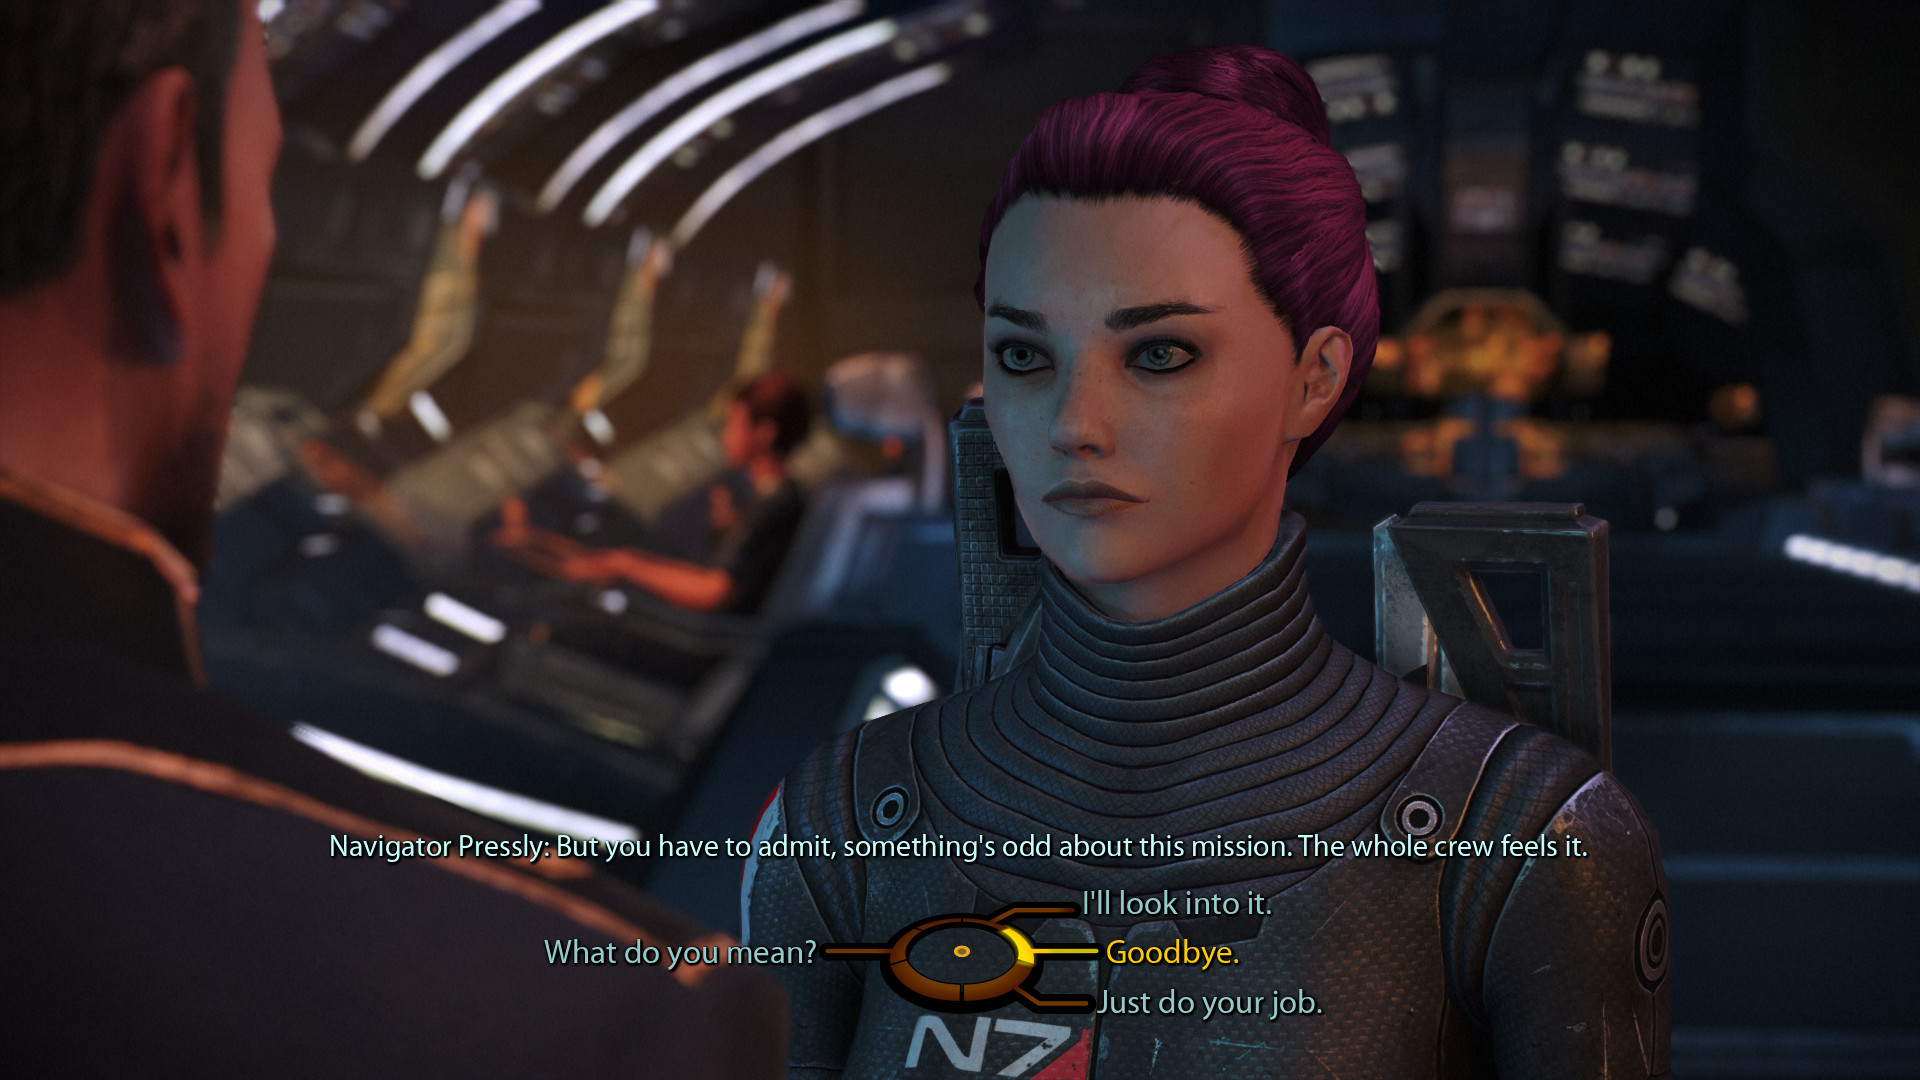
\includegraphics[width=0.6\textwidth]{images/me}
\caption{Przykład koła dialogowego w grze Mass Effect}
\label{fig:wheel}
\end{figure}
